\chapter{Data Ingestion}

When it comes to using data coming from one or more sources, being them sensors or user activities from a website, there needs to be adequate tools for handling, gathering and routing them inside the cluster where they will be processed.

\section{Apache Kafka}

\textbf{Apache Kafka} is a distributed streaming platform which lets you publish and subscribe to streams of records, similar to a message queue or enterprise messaging system, store streams of records in a fault-tolerant way and optionally process them as they occur. 

It is mainly used for building real-time streaming data pipelines that reliably get data between systems or applications and real-time streaming applications that transform or react to the streams of data.

Kafka is run on one or more servers as a cluster which stores streams of \textit{records} in categories called \textit{topics}. Each record consists of a key, a value and a timestamp.

It has two main core APIs, \textbf{Producer and Consumer API}, the basic blocks to create streams, but it's possible to use two more sets of APIs: the Streams API, which can be used to process the records and transform them from between two or more topics, and the Connector API, which allows to run producers and consumers that connect to other applications or data systems.

\subsection{Topics}

A topic is a category or feed name to which records are published. Topics in Kafka are always multi-subscriber; that is, a topic can have zero, one, or many consumers that subscribe to the data written to it.

For each topic, the Kafka cluster maintains a partitioned log, where each partition is an ordered, immutable sequence of records that is continually appended to. The records in the partitions are each assigned a sequential id number called \textit{offset} that uniquely identifies each record within the partition.

The Kafka cluster retains all published records, whether or not they have been consumed, using a configurable retention period. For example, if the retention policy is set to two days, then for the two days after a record is published, it is available for consumption, after which it will be discarded to free up space. Kafka's performance is effectively constant with respect to data size so storing data for a long time is not a cause of concerns.


\begin{figure}[h]
    \centering
    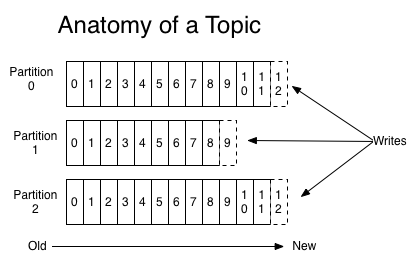
\includegraphics[width=0.7\linewidth]{Figures/log_anatomy}
    \caption[How partition works in kafka a topic]{How partition works in kafka a topic}
    \label{fig:loganatomy}
\end{figure}

The only metadata retained on a per-consumer basis is the offset or position of that consumer in the log. This offset is controlled by the consumer: normally it would advance its offset linearly as it reads records, but, in fact, it could consume records in any order it prefers. For example a consumer can reset to an older offset to reprocess data from the past or skip ahead to the most recent record and start consuming from the latest.

The partitions in the log serve several purposes. Firstly, they allow the log to scale beyond a size that will fit on a single server. Each individual partition must fit on the servers that host it, but a topic may have many partitions so it can handle an arbitrary amount of data. Secondly, they act as the unit of parallelism, more on that in a bit. This way, it's possible to increase the number of partitions of a topic as needed, according to the throughput required.

\subsection{Producers and Consumers}

\paragraph{Producers} They are the components that publish the data to the topics of their choice. They handle the assignment of each record to the partitions within the topic. This can be done according to the round-robin scheduling, to balance load, or accordingly to a semantic partition function (such it may be the key of a record).

\paragraph{Consumers} They are labelled with a \textit{consumer group} name, and each record published to a topic is delivered to one consumer instance within each subscribing consumer group. Consumer instances can be in separate processes or on separate machines.

A common configuration has topics with a small number of consumer groups, one for each "logical subscriber". Each group is composed of many consumer instances for scalability and fault tolerance, which is simple publish-subscribe semantics where the subscriber is a cluster of consumers instead of a single process.

\begin{figure}[h]
    \centering
    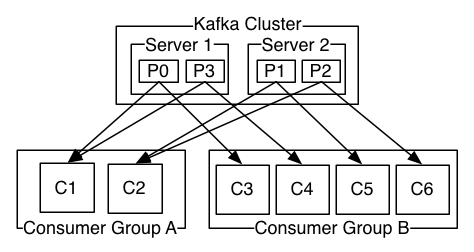
\includegraphics[width=0.7\linewidth]{Figures/consumer-groups}
    \caption[Consumer groups subscribing to a Kafka Cluster]{Consumer groups subscribing to a Kafka Cluster}
    \label{fig:consumer-groups}
\end{figure}


The way consumption is implemented in Kafka is by dividing up the partitions in the log over the consumer instances so that each instance is the exclusive consumer of a "fair share" of partitions at any point in time. This process of maintaining membership in the group is handled by Kafka dynamically, so that if new instances join the group they will take over some partitions from other members of the group, while if an instance dies, its partitions will be distributed to the remaining instances.

Kafka only provides a total order over records within a partition, not between different partitions in a topic. Per-partition ordering combined with the ability to partition data by key is sufficient for most applications. However, if a total order over records is required with a topic that has only one partition, though this will mean only one consumer process per consumer group. 

\subsection{Use cases}

\paragraph{Messaging}

Kafka can be used as a replacement for a more traditional message broker, used for reasons such as decoupling processing from data producers and buffering unprocessed messages. In comparison to most messaging systems Kafka has better throughput, built-in partitioning, replication, and fault-tolerance which makes it a good solution for large scale message processing applications.

In this domain Kafka is comparable to traditional messaging systems such as ActiveMQ or RabbitMQ. 

\paragraph{Log Aggregation}

Log aggregation typically collects physical log files off servers and puts them in a central place (a file server or HDFS perhaps) for processing. Kafka abstracts away the details of files and gives a cleaner abstraction of log or event data as a stream of messages. This allows for lower-latency processing and easier support for multiple data sources and distributed data consumption. In comparison to log-centric systems like Flume, Kafka offers equally good performance, stronger durability guarantees due to replication, and much lower end-to-end latency. 
 
\paragraph{Activity Tracking \& Metrics}

The original use case for Kafka was to be able to rebuild a user activity tracking pipeline as a set of real-time publish-subscribe feeds. This means site activity (page views, searches, or other actions users may take) is published to central topics with one topic per activity type. These feeds are available for subscription for a range of use cases including real-time processing, real-time monitoring, and loading into Hadoop or any data warehousing systems for offline processing and reporting.

Kafka is often used for operational monitoring data, aggregating statistics from distributed applications to produce centralized feeds of operational data and thus can be used as base component for a low latency fault-tolerant monitoring pipeline.


\section{Apache NiFi}

\textbf{Apache NiFi} is a distributed system for centralising, processing and distributing streams of data across a cluster. Its main feature is a web GUI allowing to visually structure the data flow directly from the sources through the definition of graphs where each vertex is called \textbf{Processor} and each edge in-between is a queue in which the \textbf{Flowfiles}, objects wrapping a single records, wait if the processor is busy.

NiFi allows for the creation of a secure cluster where each node takes care of processing a fraction of the Flowfiles circulating inside the graph, load balancing in case of node failures. 

\subsection{Processors}

As already mentioned a Processor is the basic block for the graph structure of a NiFi flow. There are a great variety of Processors built-in, ranging in function from database connections for insertions or queries and producers and consumers for queue processes such as Kafka, to object manipulation such as JSON or XML splitting and fetching and ingestion from sources like web sockets or filesystems.

A single processor can be scheduled to run periodically or continuously and can be configured with the number of concurrent tasks that need to be executed. Each Processor has different output ports according to the results of the Flowfile processing: success, failure or other processor-specific routes (e.g. \textit{\textbf{SplitText}} processor, used to split text according to user-specified rules has \textit{original} and \textit{splits} as additional output ports, used to convey in different routes Flowfiles both before and after being split).